\documentclass[a4paper,12pt]{article}
\usepackage[utf8]{inputenc}
\usepackage{graphicx}
\usepackage{hyperref}
\usepackage{listings}
\usepackage{xcolor}
\usepackage{graphicx} % Add this in the preamble



\title{React Native Lab Assignment \#3}
\author{Sowjanya Chowdary Kavuri}
\date{\today}

\begin{document}

\maketitle

\section{Screenshots of app}
\begin{enumerate}
    \item Attach screenshots of your app running on an emulator and on a physical Android or iOS device.


\includegraphics[width=0.5\textwidth]{emulator.jpeg}
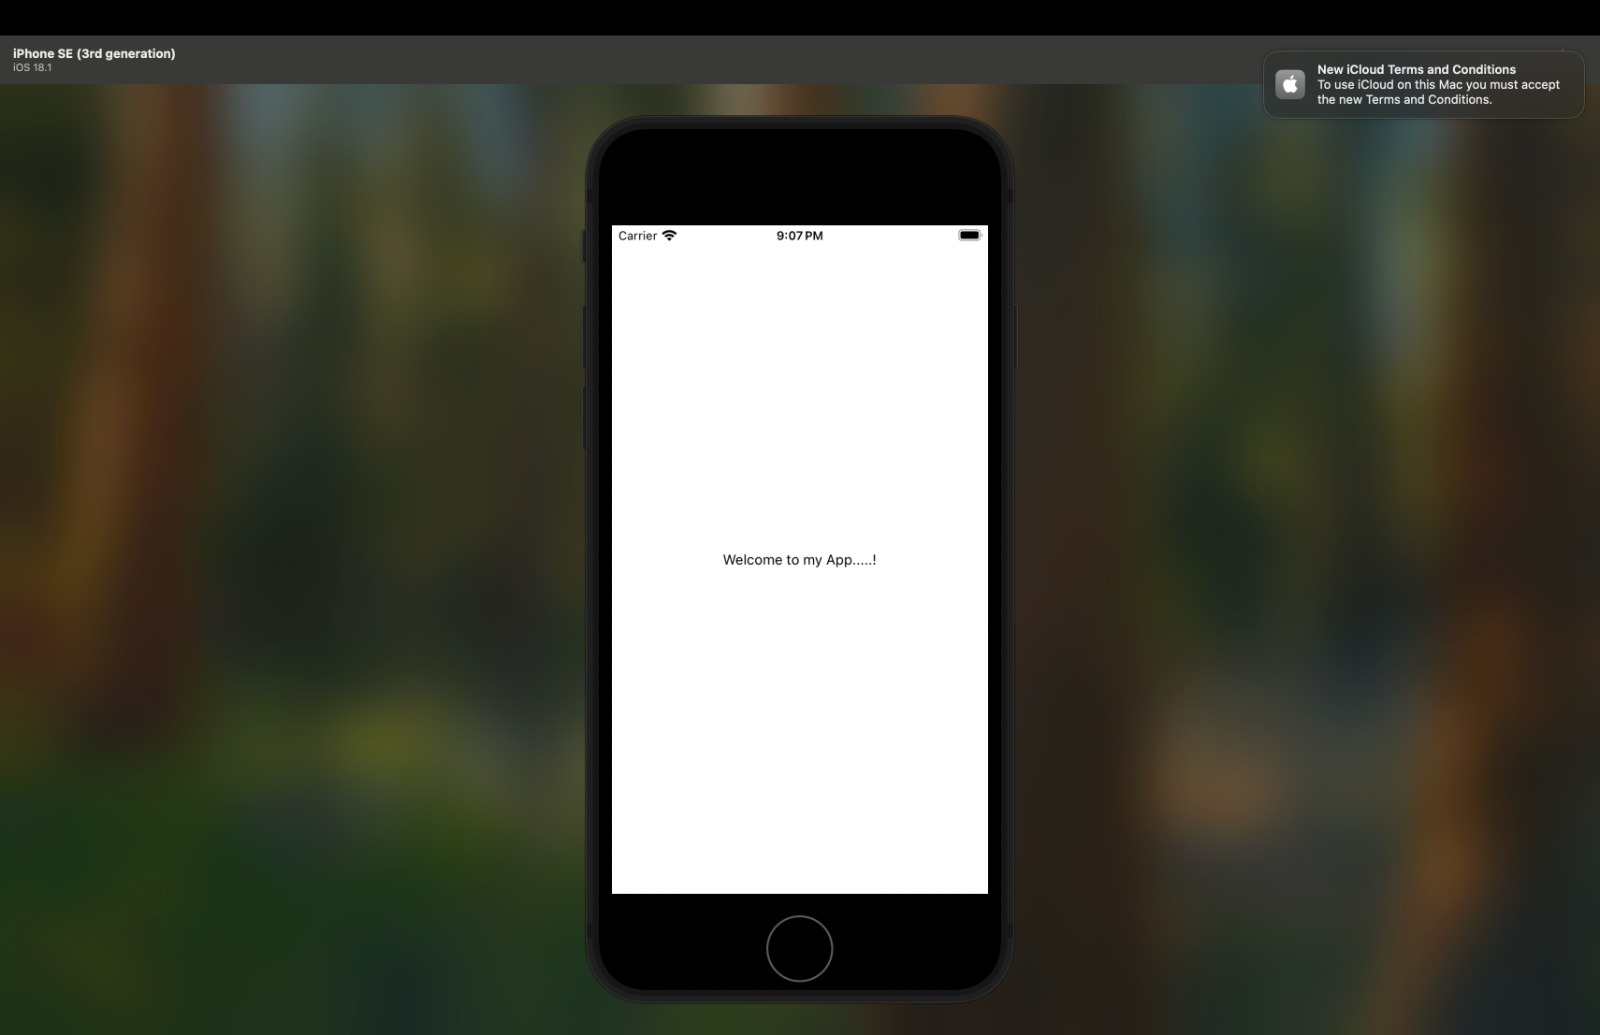
\includegraphics[width=0.5\textwidth]{phone.jpeg}

    \item Describe any differences you observed between running the app on an emulator
versus a physical device.
Both the emulator and the physical device display the text "Welcome to my App.....!" correctly.
The emulator has a simulated environment, while the physical device accurately reflects the app's appearance on a real device. Any alignment or performance issues should be more apparent on the physical device. And when the emulator is running my system experienced slow processing, took time for refreshing. For the physical device it went smoothly
\end{enumerate}

\section{Setting Up an Emulator}
\begin{enumerate}
    \item Explain the steps you followed to set up an emulator in Android Studio or Xcode.
    
    How to Configure an Emulator in Xcode
    
 1. Open the Mac App Store and install Xcode.
 
 2. From the Applications folder, launch Xcode.
 
 3. Use Preferences ¿ Components to add more simulators.
 
 4. Download the simulator of your choice (such as the iPhone SE).
 
5. Open Xcode ,Open Developer Tool ,Simulator to start the simulator.

 6. Under Hardware  Device, choose the device and iOS version.
 
 7. Click Run after opening your project in Xcode and selecting the simulator as the target.

    \item Discuss any challenges you faced during the setup and how you overcame them.
    
During the setup while installing of the xcode I didnt observed  ios got installed or not so it became an issue while running the emulator it doesn't worked and then I realised my xcode installation was not done completly other than that everything was done perfectly.Refreshing and restarting helped me well
\end{enumerate}

 \section{Running the App on a Physical Device Using Expo}

\begin{enumerate}
    \item Describe how you connected your physical device to run the app using Expo.
    On my system I runned the command npm install -g expo-cli and then Installed the Expo Go app on my physical device from the App Store.expo start it starts the development server and display a QR code in the terminal metro bundler started emulators works on,make sure both emulator and physical device connected to same wifi.Open the Expo Go app on your device.
Use the camera (on iOS) or the QR code scanner within the Expo Go app (on Android) to scan the QR code displayed in the terminal 
Run the App Once the QR code is scanned, the app will load and run on your physical device.

    \item Include any troubleshooting steps if you encountered issues
    At first I didnt got the QR code because I didnt connected the same wifi.Development Server Does Not Start,Problem: Running expo start results in an error.get rid of this issue by ensuring Node.js and npm are installed and up to date.
Clear the Expo cache using:
r
Copy code
expo start -c
\end{enumerate}

\section{Comparison of Emulator vs. Physical Device }
\begin{enumerate}
    \item Compare and contrast using an emulator versus a physical device for React Native development.
    The speed of emulator is slow when compared with the physical device and for the physical device its faster to emulator.for the emulator connection is fast but for the physical device it needs time for connecting thedevice enabling developer mode.For emulator it Can simulate multiple devices easily for physical device	Requires multiple physical devices for diverse testing


    \item Discuss the advantages and disadvantages of each option.
    
    Use an emulator when you require a cost-effective solution, for rapid iterations, or to test different screen sizes.
For precise performance testing, real-world user interaction, and when evaluating particular hardware characteristics, use a physical device.
 Emulators are convenient for quick testing.Once installed, emulators are easy to start and manage directly from your development environment.Disadvantages--Emulators may not be as fast as physical devices, especially if your system is not powerful enough. t’s difficult to replicate real touch gestures and interaction patterns, which can lead to differences in app performance and behavior when compared to a physical device.Advantages--Running the app on a real device provides an accurate representation of how the app will perform for end users.The app will run more smoothly on a physical device, as it uses the actual hardware, rather than relying on emulation software that may cause lag or reduced performance.Disadv--Setting up a physical device for testing might require additional steps, such as enabling developer mode, connecting via USB or wireless, and handling permissions.Device Availability: You need to have a physical device on hand.Slower iteration takes more time compared to an emulator where you can instantly refresh or reload.
\end{enumerate}

\section{Troubleshooting a Common Error }
\begin{enumerate}
    \item Identify a common error you encountered when starting your React Native app.Note that it is very unlikely that everyone will get the same error here.

    Unable to load the app due to the connection of development server error
    This error usually happens when there is a problem with connectivity between the app and the server or when the React Native development server is not operating correctly. It may occur for a number of reasons:

Development Server Not Running: It's possible that the Metro bundler development server has crashed or hasn't begun.
Network Problems: The application may not be able to retrieve the JavaScript bundle if the emulator or physical device is not on the same network as your development computer.
    \item Explain the cause of the error and the steps you took to resolve it.
    I checked the terminal to make sure that the Metro bundler was running by executing:

expo start

I ran the following command to clear the Metro bundler's cache:

expo start -c

I verified that both my development machine and the emulator/physical device were connected to the same Wi-Fi network.
I restarted the Wi-Fi connection or switched to a different network if there were connectivity issues.
\end{enumerate}

\section {Task 2: Building a Simple To-Do List App}

\subsection{Mark Tasks as Complete }
To update the state and reflect the completion status of tasks in the app, I implemented a completed property for each task in the tasks state. First Initially, the completed property for each task is set to false (meaning tasks are not completed when added), and then Adding a Task: When a user adds a new task, the task object is created with the completed: false property, indicating that it is not completed.Toggling the completition status This function is called when a user taps on a task to mark it as completed or incomplete.If the task is completed we apply the completed style, which adds a strikethrough effect. The key part of this feature is toggling the completed property of each task when it is clicked, then using that updated state to determine the style of the task

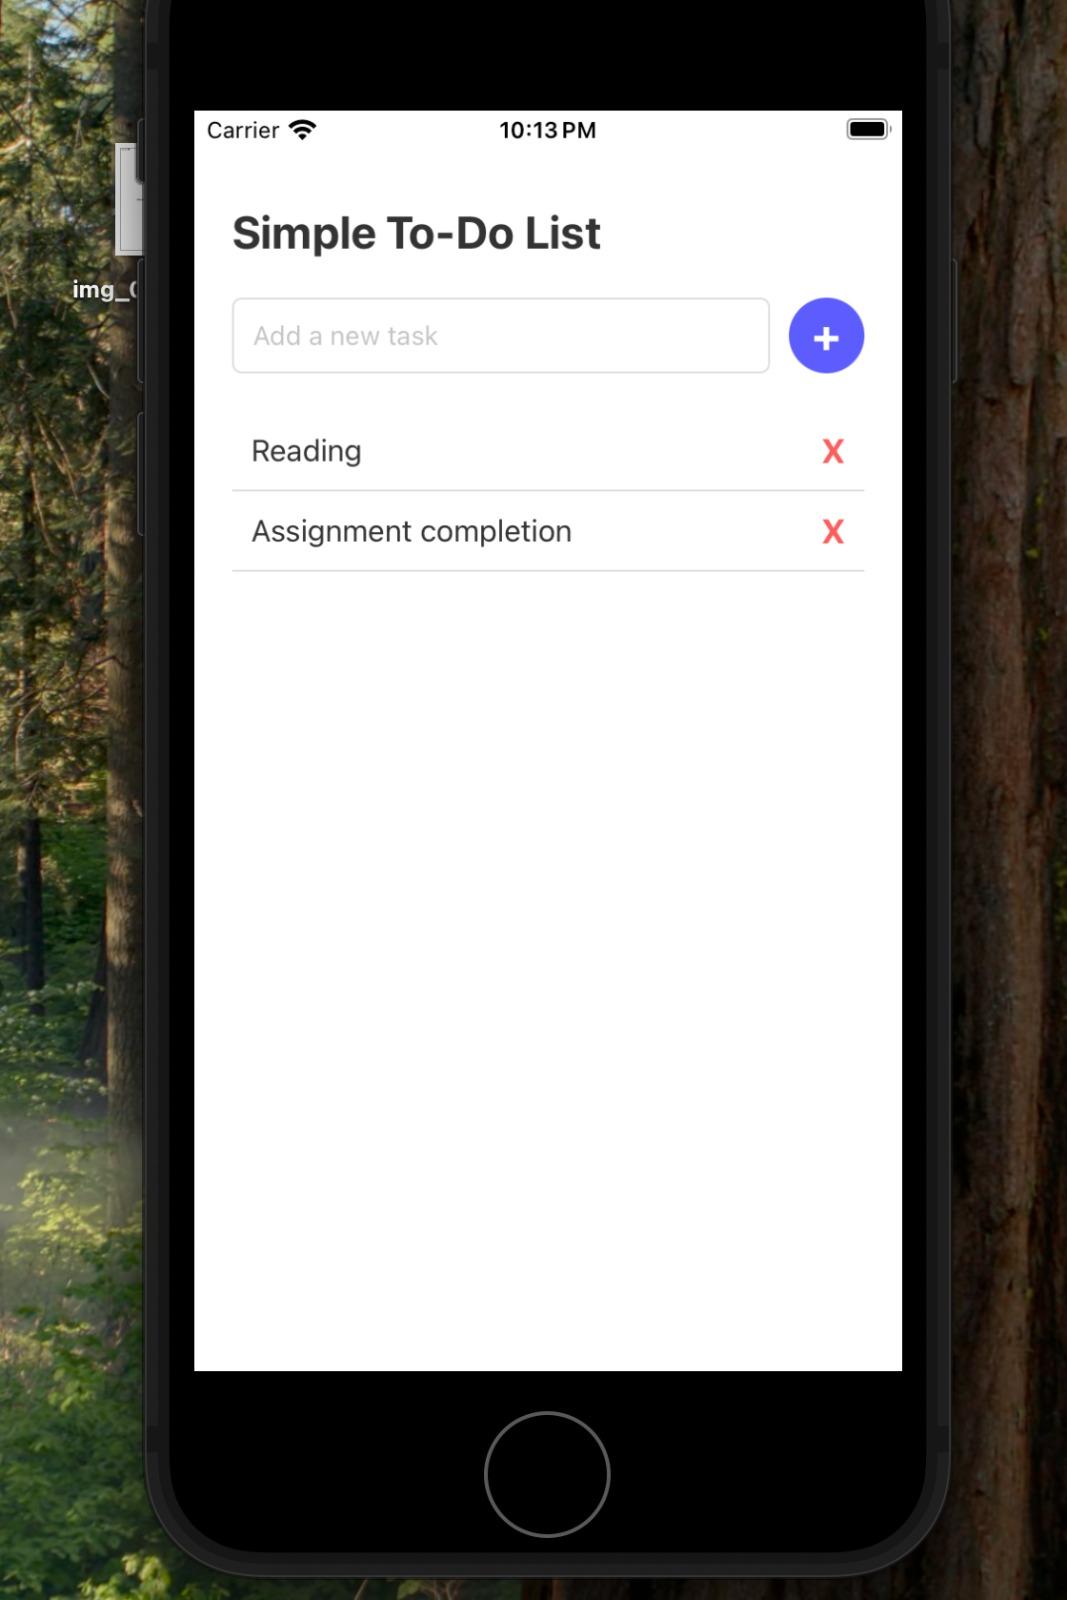
\includegraphics[width=0.5\textwidth]{task 1 a0.jpeg}
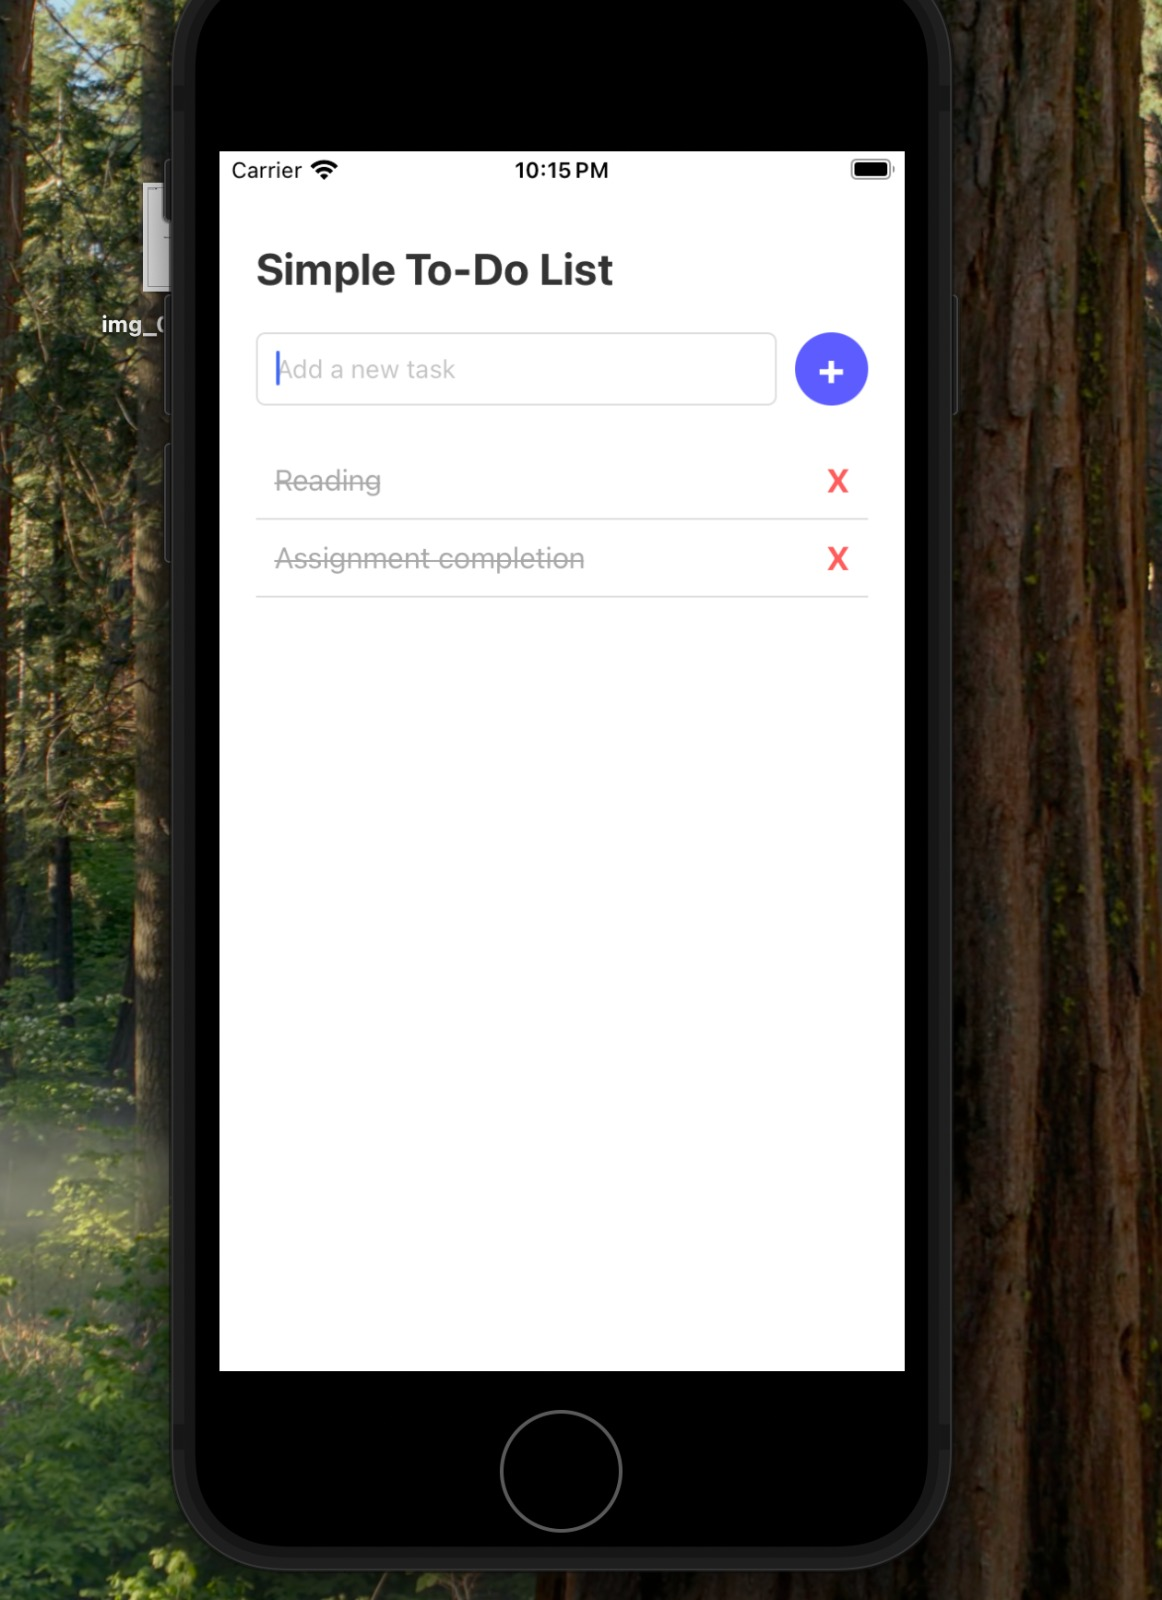
\includegraphics[width=0.5\textwidth]{task1 a.jpeg}

\subsection{Persist Data Using AsyncStorage }

useEffect hook to load tasks when the app starts, and save tasks when they change
At the top of your App.js file or the component managing the tasks, import AsyncStorage
npm install @react-native-async-storage/async-storage

 save tasks to asyncstorage
 
 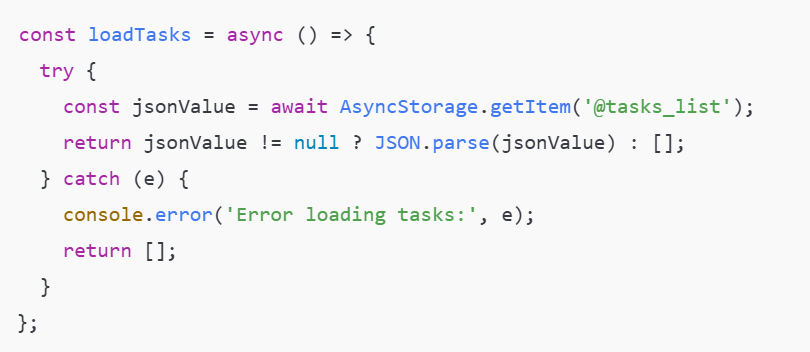
\includegraphics[width=0.5\textwidth]{per 2.png}

 To retrieve
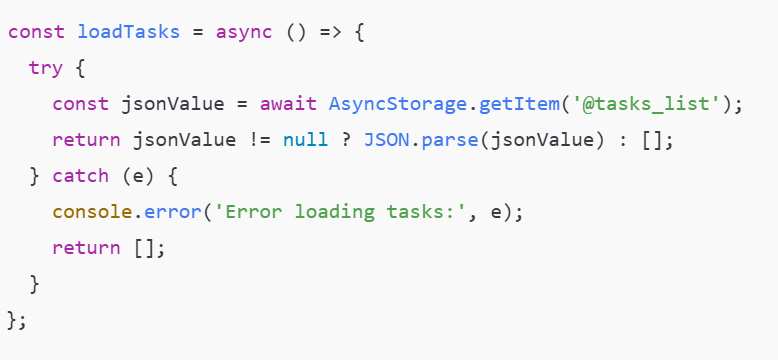
\includegraphics[width=0.5\textwidth]{per 3.png}
 



\subsection{Edit Tasks }
The user taps the "Edit" button.
The task text switches to an editable input field (TextInput).
The user types a new value.
On focus, the input closes, and the updated task text is displayed.
Each task can be toggled into an "edit mode" to enable text editing. This is done by storing the ID of the task being edited in a state variable (editMode). If editMode matches a task's ID, that task's text is replaced with a TextInput.
When not editing, tasks are displayed as regular text (Text component).
When editing, the task text is replaced by an editable input field (TextInput), allowing users to update the content.


\includegraphics[width=0.5\textwidth]{Edit task.jpeg}

\includegraphics[width=0.5\textwidth]{edit 2.jpeg}

\subsection{Add Animations }
For the animation part, fade in animation is used while adding the tasks when the new task is added it smoothly fades into the view according to the visibility I maximised and minimised the view and when deleting the tasks it fades out smoothly before the task is going to be removed

\subsection{ Git link}

https://github.com/Sowjichows/Webtech.git

\end{document} 
